\section{Course overview}

\subsection{How do different disciplines view the world?}

\begin{figure}[h]
  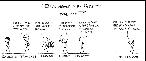
\includegraphics[width=\textwidth]{./figs/purity.pdf}
  \caption{From xkcd.com}
\end{figure}


\subsubsection{Biology}

(The focus here is on biology, but very similar comments could be made for geology and environmental science.)

Biology: The study of living organisms. The approach taken by biology is guided by and constrained by the fact that the subject is about living organisms.

\begin{enumerate}
\item Much of biology is {\bf complex}
  \begin{itemize}
    \item first steps are about identification, classification, and description of phenomena
    \item describe phenomena before looking for explanations of how it works
    \item huge vocabulary and many concepts to learn
  \end{itemize}

\item Biology depends on {\bf history}
  \begin{itemize}
  \item organisms are connected through a common, unbroken history that affects how things are today --- not the case for chemistry and physics
    \item evolution ``explains'' why a particular organism solves biological problems in a given way
  \end{itemize}
  
\item  Biology looks for {\bf mechanism}
  \begin{itemize}
    \item Not just ``What is life?'', but also and ``How does it work?''
    \item function of organs, genes, proteins and how do they affect organisms
  \end{itemize}
  
\item Biology is {\bf multi-scaled}
  \begin{itemize}
    \item organisms can be considered at many scales
    \item atomic and molecular scale (biochemistry)
    \item internal structure and functioning of organs (physiology)
    \item as part of large system in space (ecology) and time (evolution)
    \item relation between scales can be treated by reductionism or emergence --- going to smaller scales to explain something (reductionism), or seeing new phenomena arise as one goes to a larger scale (emergence)
  \end{itemize}
  
\item Biology is {\bf integrative}
  \begin{itemize}
   \item biological phenomena emerge from and must be consistent with the principles of chemistry, physics, and math
   \item chemistry and physics constrain how an organism can behave or evolve  
  \end{itemize}
\end{enumerate} 

\subsubsection{Chemistry}
Chemistry: The study of the composition and properties of substances and various elementary forms of matter.

Chemistry starts with the idea that all matter is made up of certain fundamental pieces (i.e., atoms) and is about the ways those elements combine to form more complex structures - molecules. But chemistry is not just about building molecules. It's about what you can do with that knowledge in our macroscopic world.

\begin{enumerate}
\item Chemistry is about {\bf how atoms interact to form molecules} --- Understanding the basic principles of how atoms interact and combine is a fundamental starting point for chemistry.

\item Chemistry is about {\bf developing higher-level principles and heuristics} --- Because there are so many different kinds of molecules possible, chemistry develops higher-level ideas that help you think about how complex reactions take place.

\item Chemistry frequently {\bf crosses scales}, connecting the microscopic with the macroscopic, trying to learn about molecular reactions from macroscopic observations and figuring our what is possible macroscopically from the way atoms behave. The connections are indirect, can be subtle, and may involve emergence.

\item Chemistry often assumes a {\bf macroscopic} environment --- Much of what chemistry is about is not just idealized atoms interacting in a vacuum, but is about lots of atoms interacting in an environment, such as a liquid, gas, or crystal. In a water-based environment, the availability of H$^+$ and OH$^-$ ions from the dissociation of water molecules in the environment plays an important role, while in a gas-based environment, the balance of partial pressures is critical.

\item Chemistry often {\bf simplifies} --- In chemistry, you often select the dominant reactions to consider, idealize situations and processes in order to allow an understanding of the most important features.

\end{enumerate}

For a chemist, most of what happens in biology (or geology or environmental science) is ``macroscopic'' --- there are lots and lots of atoms involved --- even though you might need a microscope to study it. In introductory chemistry you often assume that reactions are taking place at standard temperature and pressure (300 K and 1 atm).

\subsubsection{Physics}
Physics: The study of matter and its motion through space and time.

The goal of physics is to find the fundamental laws and principles that govern all matter --- including biological organisms. Those laws and principles can lead to many types of complex and apparently different phenomena.

Physics emphasizes four scientific skills that may seem different to what you see in introductory biology and chemistry classes but that are very useful:

\begin{enumerate}
\item Search for simplest possible example ({\bf ``toy model''})
  \begin{itemize}
    \item clearly illustrate key principles
    \item build-up from simple models to analyze more complex situations
  \end{itemize}
  
\item Physicists {\bf quantify} their view of the real world
  \begin{itemize}
    \item not satisfied until something can be quantified
    \item purely qualitative reasoning can be misleading
  \end{itemize}

\item Physicists {\bf think with equations}
  \begin{itemize}
    \item use equations to organize qualitative knowledge and to determine how things happen, what matters, and how much
    \item go back and forth between concepts and math
  \end{itemize}
  
\item Physicists deal with realistic situations by {\bf modeling and approximating}
  \begin{itemize}
    \item identify what matters most in a complex situation and create a ``simple'' model
    \item the art of physics: figuring out what can be ignored without losing what you want to look at
    \item ``Physics should be as simple as possible, but not simpler.''
  \end{itemize}

\end{enumerate}  

This way of doing science is a bit different from the way biology is often done --- but elements of this approach and the constraints imposed on biology by the laws of physics are becoming increasingly important.

\subsubsection{Math}
Math is a bit different from the sciences. What is math anyway??? How do mathematicians think about the world?

\begin{itemize}
  \item math is about relationships, patterns, logic
  \item abstract and rigorous
  \item not ``about'' anything in the physical world
  \item would math exist without humans?
  \item but --- a lot of relationships in science can be modeled by mathematical relationships
\end{itemize}

Math as taught in math classes often is primarily about the abstract relationships --- learning how to use the tools of math. Introductory physics is an excellent place to become comfortable with applying math to real world problems.


\subsection{Why physics?}
Why are you required to take physics?

Math majors: (1) apply your knowledge to ``real world'' problems and (2) gain an understanding of where the equations come from that you are learning how to solve and analyze

Biology / environmental science: (1) the core principles that control and organize our understanding of biology and the environment include physics and (2) the skills and competencies developed in physics are of great use in the life and environmental sciences, especially at the more advanced levels.

Useful skills that we will focus on:
\begin{enumerate}
  \item {\bf Problem solving --- modeling and mechanistic reasoning:} 
    People are needed to figure out things that are not trivially obvious. Looking at a situation that is different from one you might have seen before, finding the similarities and differences, figuring out the knowledge and tools you need to resolve it, that's problem solving. A lot of what you will learn in this class will be through problem solving. Not just learning something and giving it back, but learning something and figuring out how to use it in new non-obvious situations.

    {\it I will not expect you to memorize equations for exams, and I may ask exam questions that differ somewhat from homework assignments.}

    \item {\bf Discourse --- learning to talk the talk:} 
      A critical idea in any science is that we use the community of scientists in a discipline to get a broader, more complete, and more accurate view of the world than any one individual can get. We're each limited in our experience and knowledge. Every scientific discipline relies heavily on the interaction of scientists with each other.

      {\it We will do a lot of in-class group work, both in lab and lecture. In addition, your homework will include problems that may be too hard and time-consuming for a single individual to do easily by themselves. You are encouraged to work in groups. The point of this is for you to learn to ``talk the talk'' --- to learn to ask questions of each other until you all understand what's going on better than any of you would individually.}
      
\item {\bf Reasoning from principle:}
  Physics has been really good at finding universal (or nearly universal) principles that hold in a very wide variety of circumstances; things like energy conservation, conservation of charge, and Newton's laws --- our framework for describing and building models of motion.

  {\it By starting from basic principles and building upward, we will begin to make sense of complex knowledge in a coherent way.}

\item {\bf Quantification of experience --- mathematization, estimation, and scales:}
  All sciences are becoming increasingly quantitative. As a scientist you need to understand math and be able to interpret the implications of the math. Learning to use math in science (rather than just as pure math) can be quite tricky. Adding a physical interpretation to our symbols can actually change the way we think about the math.

{\it We'll use a lot of math of this course, so much that some of you may complain that physics is basically just another math course. In some sense that's true. We will use math to solve scientific questions, and will also learn to estimate as a way to (1) determine ``what matters most'' and (2) check that our solutions make sense.}

\item {\bf Multiple-representation translation:} 
  All sciences represent the complex information that they convey in a variety of forms -- words, equations, pictures, graphs, and animations. The tricky thing is to learn to create a single enriched physical picture in your mind that blends all these different representations, linking them together.

{\it By focusing on ``simple'' situations, we'll gain an ability to think about science from multiple perspectives. We'll make sketches of physical processes, describe the processes using equations, and interpret the equations by drawing graphs.}

\item {\bf Understanding measurement:}
  All sciences rely heavily on measurement and data, none of which is perfectly reliable. Every experiment or measurement includes some model, both of the system being measured and of the process yielding the measurements. Understanding how measurement works --- and therefore what the measurement tells you, when it can be trusted, and when it can go astray --- is very important to a practicing scientist.

  {\it We'll gain a better understanding of measurements and data through lab experiments, which will illustrate that even simple systems can involve complex issues of measurement.}
  
\end{enumerate} 

You'll also work on developing these skills in your upper-division classes. Physics is a great place to practice since physics digs down to underlying simple principles and universal constraints. The physics we are learning here is, in the end, rather simple.

%In this class we will show you how simple physical principles can also constrain complex living systems and offer simple constraints and a framework for thinking about biology. You will be introduced to a new, complementary way of thinking that will contribute to your understanding of the living world.



\clearpage
